\documentclass{article}

\usepackage[a4paper]{geometry}

\usepackage{amsmath}
\usepackage{amssymb}
\usepackage{amsthm}
\usepackage{amsfonts}
%llbracket and rrbracket
\usepackage{stmaryrd}

\usepackage[boxed,noline]{algorithm2e}

\usepackage{float}
\usepackage{tikz}

\usetikzlibrary{automata}

%Defs and thms
\theoremstyle{definition}
\newtheorem{defi}{Definition}
\newtheorem{ex}[defi]{Example}

\theoremstyle{remark}
\newtheorem{rem}[defi]{Remark}

\theoremstyle{plain}
\newtheorem{thm}[defi]{Theorem}
\newtheorem{prob}[defi]{Problem}
\newtheorem{cor}[defi]{Corollary}
\newtheorem{lem}[defi]{Lemma}

%operators
\newcommand{\val}{\operatorname{val}}
\newcommand{\until}{\ \mathcal{U}}

\tikzset{every node/.style={align=center}, >= latex, font=\scriptsize}

\newcommand{\comm}[1]{{\color{red} \marginpar{? [?]} \textsf{[#1]}}}


\title{Survey of Hybrid Automata and their Abstractions}
\author{Ruth Hoffmann}

\begin{document}
\maketitle


\begin{abstract}
With the wide applicability of hybrid systems in the real world, it is now more than ever important to be able to verify these systems for safety and reliability. This paper surveys a number of abstraction techniques which turn these continuous systems into discrete, which can be verified with a variation of tools.
\end{abstract}

\section{Introduction}
\label{sec:intro}
We model and analyse complex systems using a range of mathematical formalisms and techniques. The type of system dictates the formalism used. For example, a system exhibiting continuous behaviour (a system of chemical reactions, fluid flow, movement of an aircraft, say) can be modelled using a set of differential equations, whereas a discrete state system can be modelled as finite state transition systems (or Finite State Automata---FSAs), or as Markov chain variants. An extension to finite state automata including real-timed clocks---Timed Automata (TAs) are used to model systems with additional time-dependent behaviour, such as real time systems or networks.


Some systems exhibit both discrete and continuous behaviour and so can not be modelled as a FSA or a set of differential equations alone (for example mutual-exclusion protocols \cite{Alur1995a}, temperature regulation \cite{Nicollin1993,Amin2006,Raskin2005}, water level regulation \cite{Alur1993}, train controllers \cite{Platzer2011a}, aircraft landing \cite{Tomlin2003}, robot cooperation \cite{Chaimowicz2003} and robotic decision making \cite{Dennis2013}).
These systems are known as hybrid systems and can be modelled using hybrid automata (HAs)---where continuous behaviour is modelled using differential equations within a finite set of {\it locations} (or {\it modes}) and discrete behaviour as discrete transitions between the modes. Being able to verify a hybrid system is crucial to show that the modelled real world application is safe \cite{Livadas1998a,Prajna2007}. However, unlike FSAs, which can (at least theoretically) be analysed using explicit or symbolic search of the statespace, HAs --- thanks to their continuous component---can not (although the state reachability problem for TAs, which are a special class of HAs is decidable \cite{Alur1994}).
There are various techniques on how to build a verifiable representation of a HA, as well as numerous tools. This paper focuses on abstraction techniques, which yield a finite system, or a system that can be verified using current model checking approaches. The abstractions do not use common notation, and some are special cases. We unify these.

Other systems, in addition to continuous and discrete behaviour, have probabilistic (stochastic) attributes, and can be modelled using stochastic hybrid automata (SHAs). When this stochastic behaviour translates as probabilistic transitions between locations, the automata are known as Probabilistic Hybrid Automata (PHAs). Otherwise, the stochastic behaviour is within the locations themselves (and represented as a set of distributions).
Like HAs, the verification of SHAs requires abstraction to a simpler, verifiable form, often using techniques similar to those used for their non-stochastic counterparts.

In this paper, we survey HAs and SHAs and their abstractions. We first introduce HAs and SHAs (Sections~\ref{sec:hybrid} and \ref{sec:stoch} respectively). In Section~\ref{sec:background} we provide some additional relevant background material and in
Sections~\ref{sec:abs} and \ref{sec:propabs} we present the different abstraction techniques of HAs and PHAs respectively, and a translation of SHAs to PHAs. %Finally, in Section~\ref{sec:related} we present relevant additional related work and tools. \comm{May not need last section?}


\section{Hybrid Automata}
\label{sec:hybrid}
The formal definitions of hybrid systems vary slightly, but they all agree on the following. A hybrid system consists of continuous and discrete variables. It is represented by finite state automata, where each mode (or location) of the automaton contains continuous actions, and the transitions between modes are discrete actions. The transitions are triggered through predicates defined on the continuous or discrete variables. This representation of a hybrid system is called a hybrid automaton.

\begin{defi}[Hybrid Automaton]
A \emph{hybrid automaton} $\mathcal{A}=(V,L,A,Init,Inv,E,f)$ consists of 7 components;
\begin{description}
    \item[$V$]{Finite set of \emph{continuous variables}, with valuation $\val(V)\subseteq\mathbb{R}^n$ where $n=|V|$,}
    \item[$L$]{Finite set of \emph{locations/modes/discrete variables},}
    \item[$A$]{Finite set of \emph{actions},}
    \item[$Init$]{Set of \emph{initial states}, $Init\subseteq L \times \val(V)$,}
    \item[$Inv$]{\emph{Invariant condition}, $Inv: L \rightarrow 2^{\val(V)}$,}
    \item[$E$]{Finite set of \emph{edges}, $E\subseteq L\times A\times L$, where each edge represents a transition between two modes, and is labelled with an action and the following
        \begin{itemize}
            \item{$g : E \rightarrow 2^{\val(V)}$, a \emph{guard},}
            \item{$r : E \rightarrow 2^{\val(V)}$, a \emph{reset map},}
        \end{itemize}}
    \item[$f$]{\emph{Flow condition}, $f: L\rightarrow (\val(V)\rightarrow\val(V))$.}
\end{description}
\end{defi}

The set of states of the automaton is defined by $L\times\val(V)$. The invariant condition labels the modes with the domain of each continuous variable, while the flow function defines the behaviour of the continuous variables. For each mode $\ell\in L$ the flow of the continuous variable $x\in V$ is governed by the differential of $x$, $\dot{x}=f(\ell)(x)$.

The execution of a hybrid system, follows the semantics of the hybrid automaton, by using the set of states $L\times\val(V)$, starting in the initial states $Init$ and following two types of transitions. Firstly, the discrete transitions, which correspond to the edges $e\in E$ in the hybrid automata definition and secondly, the continuous transitions which correspond to the flow condition.

\begin{rem}[\cite{Halbwachs1994}]
The edges of the underlying automaton can be seen as transition functions, and through their reset map can change the current valuation of a continuous variable.
\end{rem}

\begin{ex}[Thermostat \cite{Henzinger2000}]
We take a simple example to illustrate a hybrid system and its corresponding automaton. Assume we have a thermostat controlling the temperature of a room. If the temperature falls beneath a certain limit, we turn the heating on, until it reaches a certain temperature. Once the upper temperature limit is reached, we turn the heating off, and so on. The automaton consists of the following $V=\{x\}$, $val(V)\subseteq\mathbb{R}$, $L=\{l_{0},l_{1}\}$, $A=\{ON,OFF\}$ and $Init=(l_{0},x\geq18)$. Each mode is labelled with the invariant condition
\begin{align*}
    Inv(l_{0}) & = \{x\geq18\} \\
    Inv(l_{1}) & = \{x\leq22\}
\end{align*}
and the flow
\begin{align*}
    f(l_{0}) & = \{\dot{x} = -0.1x\} \\
    f(l_{1}) & = \{\dot{x} = 5-0.1x\}.
\end{align*}
Finally, the edges between the modes have got guards
\begin{align*}
    g(l_{0},ON,l_{1}) & = \{x<19\}  \\
    g(l_{1},OFF,l_{0}) & = \{x>21\}
\end{align*}
and the reset maps are empty.
Figure~\ref{fig:exthermo} shows the hybrid automaton of this example, with the labelled modes and transitions.
\begin{figure}[H]
    \begin{center}
        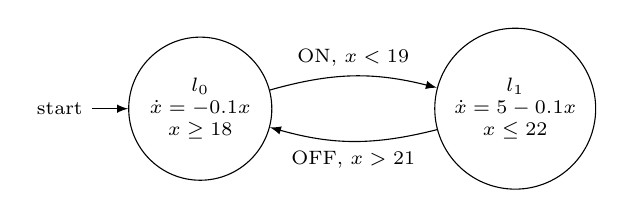
\begin{tikzpicture}[node distance=4cm]
            \node [state,initial] (s0) {$l_{0}$ \\ $\dot{x}=-0.1x$ \\ $x\geq18$};
            \node [state] (s1) [right of = s0] {$l_{1}$\\ $\dot{x}=5-0.1x$ \\ $x\leq22$};
            \path[->] (s0) edge [bend left=15] node [above] {ON, $x<19$} (s1)
                (s1) edge [bend left=15] node [below] {OFF, $x>21$} (s0);
        \end{tikzpicture}
        \caption{Hybrid Automaton of a thermostat.}
        \label{fig:exthermo}
    \end{center}
\end{figure}
\end{ex}

There are numerous types of hybrid systems which are defined by restrictions on their flow, guard and reset maps. In the next sections we are going to introduce the most common types.


%%%%%%%%%%%%%%%%%%%%%%%%%%%%%%%%%%%%%%%%%%%%%%%%%%%%%%%%%%%%%%%%%%%%%%%%%%%%%%%%%%%%%%%%%%%%%%%%%%%
%%%%%%%%%%%%%%%%%%%%%%%%%%%%%%%%%%%%%%%%%%%%%%%%%%%%%%%%%%%%%%%%%%%%%%%%%%%%%%%%%%%%%%%%%%%%%%%%%%%
%%% RECTANGULAR HA
%%%%%%%%%%%%%%%%%%%%%%%%%%%%%%%%%%%%%%%%%%%%%%%%%%%%%%%%%%%%%%%%%%%%%%%%%%%%%%%%%%%%%%%%%%%%%%%%%%%
%%%%%%%%%%%%%%%%%%%%%%%%%%%%%%%%%%%%%%%%%%%%%%%%%%%%%%%%%%%%%%%%%%%%%%%%%%%%%%%%%%%%%%%%%%%%%%%%%%%
\subsection{Rectangular Hybrid Automata}
A rectangular hybrid automaton constricts the behaviour of the continuous variables within the modes. The slope of the continuous variables in each mode can vary within a bounded or unbounded rational interval.
%\cite{Puri1994} \cite{Henzinger1995}

\begin{defi}[Rectangular Set]
For $\mathbb{R}^{n}$, with variables $x_{1},\ldots,x_{n}$, a \emph{rectangular set} is a conjuction of linear inequalities such as $x_{i}\sim c$, where $\sim\in\{<,\leq,=,\geq,>\}$, and $c\in\mathbb{Q}$. We say that for a rectangular set $R$, $R_{i}$ is the projection of $R$ onto $x_{i}$. So a rectangular set $R\subseteq\mathbb{R}^{n}$ is of the form $R=R_{1}\times\cdots\times R_{n}$.
\end{defi}

\begin{defi}[Rectangular Automaton]
A hybrid automaton $\mathcal{A} = (V,L,A,Init,Inv,E,f)$ is \emph{rectangular} if
\begin{itemize}
    \item{for every $\ell\in L$ the sets $Init(\ell)$ and $Inv(\ell)$ are rectangular,}
    \item{for every $\ell\in L$, there is a rectangular set $R^{\ell}$ such that $f(\ell)(x)=R^{\ell}$, $\forall x \in V$,}
    \item{and on every edge $e\in E$ the guard set $g(e)$, and reset map $r(e)$ are rectangular.}
\end{itemize}
\end{defi}

\begin{ex}[Rectangular Automaton Example \cite{Alur2000}]
Figure~\ref{fig:exrect} shows a generic example of a rectangular hybrid automaton. The slopes of the differential equations are within a given bound and all sets in the modes and on the edges are rectangular.
\begin{figure}[H]
    \begin{center}
        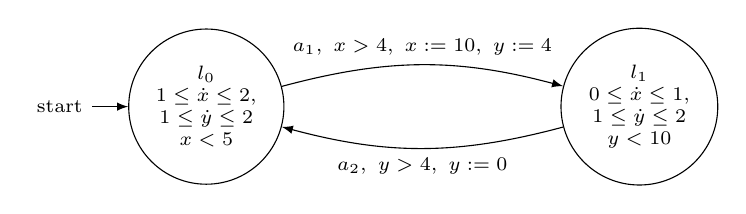
\begin{tikzpicture}[node distance=5.5cm]
            \node [state,initial] (s0) {$l_{0}$ \\ $1\leq\dot{x}\leq2,$\\$1\leq\dot{y}\leq2$ \\ $x<5$};
            \node [state] (s1) [right of = s0] {$l_{1}$ \\ $0\leq\dot{x}\leq1,$\\$1\leq\dot{y}\leq2$ \\ $y<10$};
            \path[->] (s0) edge [bend left=15] node [above] {$a_{1},\ x>4,\ x:=10,\ y:=4$} (s1)
                (s1) edge [bend left=15] node [below] {$a_{2},\ y>4,\ y:=0$} (s0);
        \end{tikzpicture}
        \caption{Example of a rectangular automaton.}
        \label{fig:exrect}
    \end{center}
\end{figure}
\end{ex}


%%%%%%%%%%%%%%%%%%%%%%%%%%%%%%%%%%%%%%%%%%%%%%%%%%%%%%%%%%%%%%%%%%%%%%%%%%%%%%%%%%%%%%%%%%%%%%%%%%%
%%%%%%%%%%%%%%%%%%%%%%%%%%%%%%%%%%%%%%%%%%%%%%%%%%%%%%%%%%%%%%%%%%%%%%%%%%%%%%%%%%%%%%%%%%%%%%%%%%%
%%% LINEAR HA
%%%%%%%%%%%%%%%%%%%%%%%%%%%%%%%%%%%%%%%%%%%%%%%%%%%%%%%%%%%%%%%%%%%%%%%%%%%%%%%%%%%%%%%%%%%%%%%%%%%
%%%%%%%%%%%%%%%%%%%%%%%%%%%%%%%%%%%%%%%%%%%%%%%%%%%%%%%%%%%%%%%%%%%%%%%%%%%%%%%%%%%%%%%%%%%%%%%%%%%
\subsection{Linear Hybrid Automata}
The characteristics of a linear hybrid automaton are the linear expressions of the continuous variables. \cite{Alur1995a} Linear automata are also called \emph{multirate automata} \cite{Alur1995a,Alur2000}.

\begin{defi}[Linear Term \cite{Henzinger2000}]
Let $k_{0},\ldots,k_{n}\in \mathbb{Z}$, and $x_{0},\ldots,x_{n}\in V$ with $val(V)\subseteq \mathbb{R}^n$, be integer parameters and real valued variables, then the \emph{linear term} is
\[
k_{0}x_{0} + \cdots + k_{n}x_{n}.
\]
\end{defi}

\begin{defi}[Linear Hybrid Automaton \cite{Henzinger2000}]
A hybrid automaton $\mathcal{A}=(V,L,A,Init,Inv,E,f)$ is \emph{linear} if
\begin{itemize}
    \item{$Init, Inv, g, r$ are boolean combinations of the form $\tau_{1} \sim \tau_{2}$, where $\sim\in\{<,\leq,=,\geq,>\}$ and $\tau_{1},\tau_{2}$ are linear terms over $V$.}
    \item{and if the flow condition is of the form $f(l)=\{\dot{x}=k : x\in V,\ k\in\mathbb{Z}\}$, for $l\in L$, $x\in V$.}
\end{itemize}
\end{defi}

\begin{ex}[Water-level monitor \cite{Halbwachs1994}]
The water level in a tank is observed by a monitor, which operates a pump. While the pump is off, the water level in the tank drops by a certain rate, should the level fall beneath a certain threshold the monitor signals the pump, which then turns on. While the pump is on, the water level in the tank increases up to a certain certain volume, when it is reached the monitor sends signal to the pump to turn it off.
\begin{figure}[H]
    \begin{center}
        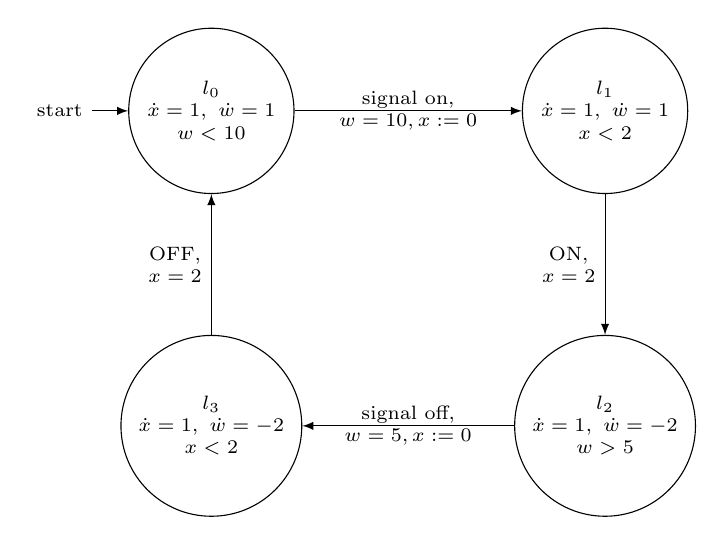
\begin{tikzpicture}[node distance=5cm]
            \node[state,initial] (s0) {$l_{0}$ \\ $\dot{x}=1,\ \dot{w}=1$ \\ $w<10$};
            \node[state] (s1) [right of = s0] {$l_{1}$ \\ $\dot{x}=1,\ \dot{w}=1$ \\ $x<2$};
            \node[state] (s2) [below of = s1,node distance=4cm] {$l_{2}$ \\ $\dot{x}=1,\ \dot{w}=-2$ \\ $w>5$};
            \node[state] (s3) [below of = s0,node distance=4cm] {$l_{3}$ \\ $\dot{x}=1,\ \dot{w}=-2$ \\ $x<2$};
            \path[->] (s0) edge node {signal on, \\ $w=10,x:=0$} (s1)
                (s1) edge node [left] {ON, \\ $x=2$} (s2)
                (s2) edge node {signal off, \\ $w=5,x:=0$} (s3)
                (s3) edge node [left] {OFF, \\ $x=2$} (s0);
        \end{tikzpicture}
        \caption{Linear Hybrid Automaton of a water-level monitor.}
        \label{fig:exwaterlevel}
    \end{center}
\end{figure}
\end{ex}
Another way of looking at linear hybrid automata is as this type being a special case of rectangular automata.

\begin{defi}[Linear Hybrid Automaton \cite{Alur2000}]
A \emph{linear hybrid automaton} is a rectangular automaton where
\begin{itemize}
    \item{for each $\ell\in L$, $Init(\ell)$ is a singleton or empty, $R^{\ell}=f(\ell)(x)$ is a singleton set, $\forall x\in V$,}
    \item{for each edge $e\in E$ the guard set $g(e)$ and the reset map $r(e)$ are singleton sets.}
\end{itemize}
\end{defi}

\subsection{Timed Automata}
Timed automata were originally introduced as timed B\"{u}chi Automata \cite{Alur1990,Alur1994}, and can be seen as a special case of linear hybrid automata.

\begin{defi}[Timed Automaton \cite{Lygeros2004}]
A \emph{timed automaton} is a linear hybrid automaton where the flow condition in all modes is of the form $\dot{x}=1$, $\forall x\in V$.
\end{defi}

\begin{ex}[Timed Automaton Example \cite{Alur2000}]
The automaton in Figure~\ref{fig:extime} is a generic example of a timed automaton. The automaton is similar to the example of a rectangular automaton in Figure~\ref{fig:exrect}. Noticeable are the differential equations which in the timed automaton ate all of the form $\dot{x}=1$.

\begin{figure}[H]
    \begin{center}
        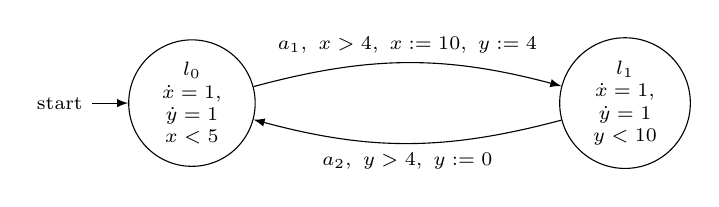
\begin{tikzpicture}[node distance=5.5cm]
            \node [state,initial] (s0) {$l_{0}$ \\ $\dot{x}=1,$\\$\dot{y}=1$ \\ $x<5$};
            \node [state] (s1) [right of = s0] {$l_{1}$ \\ $\dot{x}=1,$\\$\dot{y}=1$ \\ $y<10$};
            \path[->] (s0) edge [bend left=15] node [above] {$a_{1},\ x>4,\ x:=10,\ y:=4$} (s1)
                (s1) edge [bend left=15] node [below] {$a_{2},\ y>4,\ y:=0$} (s0);
        \end{tikzpicture}
        \caption{Example of a timed automaton.}
        \label{fig:extime}
    \end{center}
\end{figure}
\end{ex}


%%%%%%%%%%%%%%%%%%%%%%%%%%%%%%%%%%%%%%%%%%%%%%%%%%%%%%%%%%%%%%%%%%%%%%%%%%%%%%%%%%%%%%%%%%%%%%%%%%%
%%%%%%%%%%%%%%%%%%%%%%%%%%%%%%%%%%%%%%%%%%%%%%%%%%%%%%%%%%%%%%%%%%%%%%%%%%%%%%%%%%%%%%%%%%%%%%%%%%%
%%% STOCHASTIC HA
%%%%%%%%%%%%%%%%%%%%%%%%%%%%%%%%%%%%%%%%%%%%%%%%%%%%%%%%%%%%%%%%%%%%%%%%%%%%%%%%%%%%%%%%%%%%%%%%%%%
%%%%%%%%%%%%%%%%%%%%%%%%%%%%%%%%%%%%%%%%%%%%%%%%%%%%%%%%%%%%%%%%%%%%%%%%%%%%%%%%%%%%%%%%%%%%%%%%%%%
\subsection{Stochastic Hybrid Automata}

One type of stochastic hybrid automata is governed by stochastic behaviour of the continuous variables in each mode, rather than deterministic behaviour. So the flow of the continuous variables in the modes evolves through stochastic differential equations
\[
\dot{x} = f(\ell)(x) + dB_{t},
\]
where $B_{t}$ can be seen as the standard Brownian motion in $\mathbb{R}$ \cite{Hu2000}, or as a $\mathbb{R}^{n}$ valued Wiener process \cite{Koutsoukos2006}.

Further, the transitions between the modes will be probabilistic.

\begin{defi}[Stochastic Hybrid Automaton \cite{Hu2000}]
A \emph{stochastic hybrid automaton} is a hybrid automaton $\mathcal{A}=(V,L,A,Init,Inv,E,f)$ where
\begin{itemize}
    \item{for each edge $e\in E$ the guard $g(e)$ is a measurable subset of $\delta Inv$, or empty,}
    \item{the reset map $r$ is changed to be $r : E \rightarrow \mathcal{P}(val(V))$, such that is assigns each edge $(\ell,a,\ell')\in E$ a reset probability kernel on $val(V)$ concentrated on $Inv(\ell')$. Further, for any measurable set $M\subset Inv(\ell')$, $r(e)(M)$ is a measurable function.}
\end{itemize}
\end{defi}

\begin{ex}[Car Chase \cite{Hu2000}]
Imagine two cars $x_{1}$ and $x_{2}$ on a straight road. Both cars drive in the same direction, where the task for $x_{1}$ is to catch up with $x_{2}$ (which is driving at a constant speed) up to given distance, keep following, if $x_{1}$ gets too close, $x_{1}$ breaks and falls back. The motion of both cars is stochastic, due to many unknown factors such as the road condition or the environment. We can abstract the stochastic behaviour away from the motion of $x_{2}$ as we are modeling the behaviour of $x_{1}$. The distance between the two cars is $\Delta x$. There are multiple distance thresholds we consider $d_{0}>d_{1}>d_{2}>d_{3}>0$ which are in order, post breaking distance, chasing distance, keeping distance and being too close. Figure~\ref{fig:excar} shows the three modes of the scenario, chasing, keeping up and breaking. We denote the probability of $x_{1}$ falling behind $x_{2}$ further than the the keeping up distance by $p$, so the probability of being too close to $x_{2}$ is $1-p$.
\begin{figure}[H]
    \begin{center}
        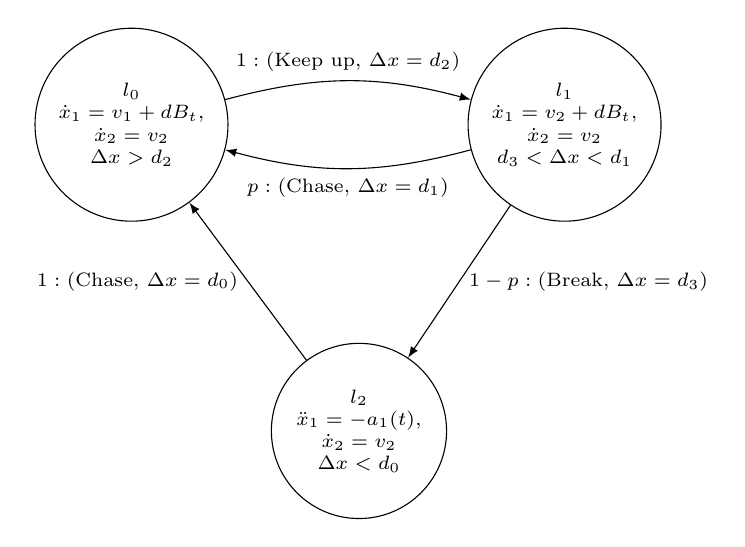
\begin{tikzpicture}[node distance=5.5cm]
            \node [state] (s0) {$l_{0}$\\ $\dot{x}_{1}=v_{1}+dB_{t},$\\$\dot{x}_{2}=v_{2}$\\ $\Delta x>d_{2}$};
            \node [state] (s1) [right of = s0] {$l_{1}$\\ $\dot{x}_{1}=v_{2}+dB_{t},$\\$\dot{x}_{2}=v_{2}$\\ $d_{3}<\Delta x<d_{1}$};
            \node [state] (s2) [below right of = s0,xshift=-1cm] {$l_{2}$\\ $\ddot{x}_{1}=-a_{1}(t),$\\$\dot{x}_{2}=v_{2}$\\ $\Delta x<d_{0}$};
            \path[->] (s0) edge [bend left=15] node [above] {$1:($Keep up, $\Delta x=d_{2})$} (s1)
                (s1) edge [bend left=15] node [below] {$p:($Chase, $\Delta x=d_{1})$} (s0)
                    edge node [right] {$1-p:($Break, $\Delta x=d_{3})$} (s2)
                (s2) edge node [left] {$1:($Chase, $\Delta x=d_{0})$} (s0);
        \end{tikzpicture}
        \caption{Example of a simplistic car chase as a stochastic hybrid automaton.}
        \label{fig:excar}
    \end{center}
\end{figure}
\end{ex}

Another type of stochastic hybrid systems have just probabilistic discrete transitions between the modes, while the behaviour of the continuous variables inside the modes can be deterministic. This type of hybrid automaton is called probabilistic.

\begin{defi}[Probabilistic Hybrid Automaton \cite{Hahn2011}]
A hybrid automaton $\mathcal{A}=(V,L,A,Init,Inv,E,f)$ is \emph{probabilistic} if we define a \emph{transition function} on the edges between the modes $t : L\times A \rightarrow \mathcal{P}(L)$, where $\mathcal{P}(L)$ is a distribution over $L$, and the guard and reset maps, $g(\ell,a,\ell'),\ r(\ell,a,\ell')$  are defined over the set of edges $E \subseteq L \times A \times L$ if $t(\ell,a)=\mathcal{P}(\ell')\neq 0$.
\end{defi}


%%%%%%%%%%%%%%%%%%%%%%%%%%%%%%%%%%%%%%%%%%%%%%%%%%%%%%%%%%%%%%%%%%%%%%%%%%%%%%%%%%%%%%%%%%%%%%%%%%%
%%%%%%%%%%%%%%%%%%%%%%%%%%%%%%%%%%%%%%%%%%%%%%%%%%%%%%%%%%%%%%%%%%%%%%%%%%%%%%%%%%%%%%%%%%%%%%%%%%%
%%% O MIN HA
%%%%%%%%%%%%%%%%%%%%%%%%%%%%%%%%%%%%%%%%%%%%%%%%%%%%%%%%%%%%%%%%%%%%%%%%%%%%%%%%%%%%%%%%%%%%%%%%%%%
%%%%%%%%%%%%%%%%%%%%%%%%%%%%%%%%%%%%%%%%%%%%%%%%%%%%%%%%%%%%%%%%%%%%%%%%%%%%%%%%%%%%%%%%%%%%%%%%%%%
\subsection{Order-Minimal Hybrid Automata}
The idea behind order-minimal hybrid automata is to limit the discrete transitions, rather than the continuous flow. With this restriction it can be easier to abstract the hybrid system.

%To introduce the notion of order-minimality, first we need to consider a few definitions from formal language theory.

%\begin{defi}[Theory]

%\end{defi}

\begin{defi}[Order-Minimal Theory \cite{Lafferriere1999}]
The theory over the reals $Th(\mathbb{R})$ is \emph{o-minimal} (order-minimal) if every definable subset of $\mathbb{R}$ is a finite union of points and intervals (possibly unbounded).
\end{defi}

\begin{defi}[Order-Minimal Hybrid Automaton \cite{G.Lafferiere2000}]
A hybrid system $\mathcal{A}=(V,L,A,Init,Inv,E,f)$ is called \emph{o-minimal} if
\begin{itemize}
    \item{for each $\ell\in L$, the flow $f(\ell)$ is a complete differential function (defined for all time);}
    \item{for each $e\in E$, the reset map $r(e)$ is a piecewise constant but set valued map, with a finite number of pieces;}
    \item{for each $\ell\in L$ and all $e\in E$, $Inv(\ell),\ Init(\ell),\ , g(e),\ f(\ell)$ are definable over the same o-minimal theory over $\mathbb{R}$.}
\end{itemize}
\end{defi}

\begin{ex}[Timed Digital Code \cite{Brihaye2005}]
In this example we model a door which is locked and alarmed. To unlock it safely the user has to swipe a card $c$ and then enter the correct passcode $w$. The passcode is $ABC$ and the user has one time unit $t$ for each letter. Should they enter a wrong letter or not within the given time, the alarm will go off. This example can be modelled as a o-minimal hybrid automaton as in Figure~\ref{fig:expass}.

\begin{figure}[H]
    \begin{center}
        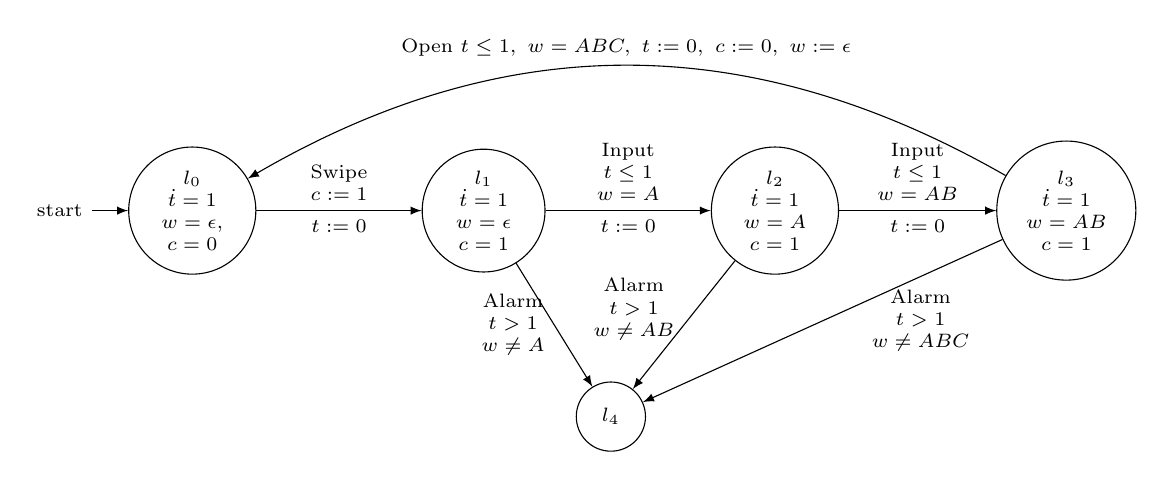
\begin{tikzpicture}[node distance=3.7cm]
            \node [state,initial] (s0) {$l_{0}$\\$\dot{t}=1$\\$w=\epsilon,$\\$c=0$};
            \node [state] (s1) [right of = s0] {$l_{1}$\\$\dot{t}=1$\\$w=\epsilon$\\$c=1$};
            \node [state] (s2) [right of = s1] {$l_{2}$\\$\dot{t}=1$\\$w=A$\\$c=1$};
            \node [state] (s3) [right of = s2] {$l_{3}$\\$\dot{t}=1$\\$w=AB$\\$c=1$};
            \node [state] (s4) [below right of = s1,xshift=-1cm] {$l_{4}$};

            \path[->] (s0) edge node [above] {Swipe\\$c:=1$} node [below] {$t:=0$} (s1)
                (s1) edge node [above] {Input\\$t\leq1$\\$w=A$} node [below] {$t:=0$} (s2)
                    edge node [left] {Alarm\\$t>1$\\$w\neq A$} (s4)
                (s2) edge node [above] {Input\\$t\leq1$\\$w=AB$} node [below] {$t:=0$} (s3)
                    edge node [left,yshift=2mm] {Alarm\\$t>1$\\$w\neq AB$} (s4)
                (s3) edge [bend right] node [above] {Open $t\leq1,\ w=ABC,\ t:=0,\ c:=0,\ w:=\epsilon$} (s0)
                    edge node [right,xshift=5mm] {Alarm\\$t>1$\\$w\neq ABC$} (s4);

        \end{tikzpicture}
        \caption{Example of a secured door, with timed passcode entry.}
        \label{fig:expass}
    \end{center}
\end{figure}
\end{ex}

Rectangular Set: conjunction of $x\sim c$, where $x\in \val(C)$, $c\in\mathbb{Q}$, and $\sim\in\{<,\leq,=,\geq,>\}$; $B=B_{1}\times\cdots\times B_{n}\subseteq \mathbb{R}^{n}$.

Linear Term: $k_{0}x_{0}+\cdots+k_{n}x_{n}$, where $k_{0},\ldots,k_{n}\in \mathbb{Z}$, $x_{0},\ldots,x_{n}\in V$, $\val(V)\in\mathbb{R}^{n}$.
Linear Expression: $\tau_{1}\sim\tau_{2}$, where $\sim\in\{<,\leq,=,\geq,>\}$ and $\tau_{1},\tau_{2}$ are linear terms.



\begin{table}
\begin{center}
\begin{tabular}{|l|l|l|l|l|}\hline
Type & $Init$, $Inv$ & $g$ & $r$ & $f$ \\ \hline
Rectangular & Rectangular & Rectangular & Rectangular & $f(\ell)(x) = B^{\ell}$ \\ \hline
Linear & Linear & Linear  & Linear  & $f(\ell)(x)=k$ \\ \hline
Timed & Linear & Linear & Linear & $f(\ell)(x)=1, \forall x$ \\ \hline
Stochastic &  &  &  & \\ \hline
O-Minimal &  &  &  & \\ \hline
\end{tabular}
\label{tab:hasummary}
\caption{Summary of the presented types of hybrid systems.}
\end{center}
\end{table}
%\cite{Alur1995a,Amin2006,Alur1993,Alur2011a,Henzinger2000,Maler2014a,Nicollin1993,Platzer2011a,Raskin2005,Tabuada,Fehnker2004,Tomlin2003,Alur1997,Asarin1997}

%\cite{Alur2011a} mentions some abstractions  (flowpipe, simulation, phase portrait)

%\cite{Henzinger2000} covers some abstraction techniques with refs (discrete, bisimulation, $\mu$)

%\cite{Maler2014a} contains some refs to different types of abstr.

%\cite{Asarin1997} timed aut abstraction using numberical decision diagram

%\subsection{Applications}
%\cite{Chaimowicz2003} in robotic cooperation

%\cite{Dennis2013a} more robotic applications and some refs to abstractions.

%\cite{Fehnker2004} contains benchmarks and uses both d/dt anf charon.

%\cite{Tomlin2003} with tools


\section{Abstractions}
\label{sec:abs}
We introduce the bisimulation of non-probabilistic systems, as it can be used on the underlying non-deterministic structure of a PHA to determine whether the PHA can be abstracted. A bisimulation is a property preserving equivalence relation on the states.

A hybrid system $\mathcal{A}=(V,L,A,\Init,Inv,E,f)$ generates a transition system $\mathcal{T}_{\Sigma,\mathcal{A}}=(Q,Q_{0},\Pi,t,\models)$ according to a finite set of subsets of $\mathbb{R}^{n}$, denoted $\Sigma$, where $n$ is the number of continuous variables \cite{Alur2000}. Then
\begin{itemize}
\item{$Q=L\times \val(V)$ is the set of states;}
\item{$Q_{0}=\Init$ is the set of initial states;}
\item{$\Pi=L\cup\Sigma$ is the set of propositions;}
\item{$(\ell,x)\models\pi$ is the satisfaction relation where $\ell\in L$ and then $\pi\in L$ if and only if $\ell = \pi$, or $\pi\in\Sigma$ if and only if $x\in\pi$;}
\item{$t=(\bigcup_{e\in E}\overset{e}{\rightarrow})\cup \overset{\tau}{\rightarrow}$ is the
transition function, with each $\overset{e}{\rightarrow}$ being the discrete transitions, which are
defined as $(\ell,x)\overset{e}{\rightarrow}(\ell',x')$ for $e=(\ell,a,\ell')\in E$ for any
$a\in A$ if and only if $x\in g(e)$ and $x' \in r(e)$ and $\overset{\tau}{\rightarrow}$ are
continuous transitions, which are defined as
$(\ell_{1},x_{1})\overset{\tau}{\rightarrow}(\ell_{2},x_{2})$ if and only if $\ell_{1}=\ell_{2}$,
and $\exists \delta \in \mathbb{R}^{+}\setminus\{ 0\}$ and there is a differentiable curve
$x:[0,\delta]\rightarrow \mathbb{R}^{n}$ with $x(0)=x_{1}$, $x(\delta)=x_{2}$ and
$\forall t\in[0,\delta]$ $x(t)\in Inv(\ell_{1})$, $\forall t\in (0,\delta)$
$\dot{x}(t)\in f(\ell_{1})$ .}
\end{itemize}


We need to show that the constructed transition system still preserves the properties accordingly. For that we are looking at bisimulations to show that in fact we can still check CTL or LTL properties, through partitioning the state space.

\begin{defi}[Equivalence Relation on States]
An \emph{equivalence relation} $\sim\subseteq Q\times Q$ on the state space of a transition system $\mathcal{T}$ is a proposition preserved for all states $p,q\in Q$ and all propositions $\pi\in\Pi$, if $p\sim q$ and $p\models\pi$, then $q\models\pi$.
\end{defi}

So $\llbracket \pi\rrbracket$, the set of states satisfying the property $\pi$, can be seen as the union of equivalence classes.

\begin{defi}[Quotient Transition System]
Given a proposition preserving equivalence relation $\sim$, a \emph{quotient transition system} $\mathcal{T}/_{\sim}=(Q/_{\sim},Q_{0}/_{\sim},\Pi,t_{\sim},\models_{\sim})$ consists of
\begin{itemize}
\item{$Q/_{\sim}$ the quotient space, the set of equivalence classes;}
\item{$t_{\sim}$ the transition relation, for $P_{1},P_{2}\in Q/_{\sim}$ we have $t_{\sim}(P_{1})=P_{2}$ if and only if there exists two states $q_{1}\in P_{1}$ and $q_{2}\in P_{2}$ such that $t(q_{1})=q_{2}$.}
\item{$\models_{\sim}$ the satisfaction relation, where for $P\in Q/_{\sim}$ $P\models_{\sim}\pi$ if and only if $\exists p\in P$ such that $p\models \pi$.}
\end{itemize}
\end{defi}

For any set of states $P$, let $P/_{\sim}$ denote the collection of all equivalence classes that intersect $P$.

\begin{defi}[Bisimulation \cite{Roggenbach2000}]
Let $\mathcal{T}=(Q,Q_{0},\Pi,t,\models)$ be a transition system. A proposition preserving equivalence relation $\sim_{B}$ on $Q$ is a \emph{bisimulation} of $\mathcal{T}$ if for all states $p,q\in Q$ if $p \sim_{B} q$, then for all states $p'\in Q$ if $t(p)=p'$, $\exists q'\in Q$ such that $t(q)=q'$ and $p'\sim_{B} q'$.
\end{defi}

If $\sim_{B}$ is a bisimulation, then the quotient transition system $\mathcal{T}/_{\sim_{B}}$is called a \emph{bisimulation quotient} of $\mathcal{T}$.

\begin{thm}[\cite{Browne1988}]
Let $\mathcal{T}$ be a transition system and let $\sim_{B}$ be a bisimulation of $\mathcal{T}$. Then $\mathcal{T}$ satisfies the CTL formula $\phi$ if and only if the bisimulation quotient $\mathcal{T}/_{\sim_{B}}$ satisfies $\phi$.
\end{thm}

We can construct the bisimulation quotient algorithmically, as shown in Algorithm~\ref{alg:bisim}.

\begin{algorithm}[H]
$Q/_{\sim_{B}} := \{ \llbracket \pi \rrbracket : \pi \in \Pi\}$\;
\While{$\exists P,P'\in Q/_{\sim_{B}}$ such that $\emptyset\subset P\cap Pre(P')\subset P$}{
    $P_{1}:=P\cap Pre(P')$\;
    $P_{2}:=P\setminus Pre(P')$\;
    $Q/_{\sim_{B}}:=(Q/_{\sim_{B}}\setminus\{P\})\cup\{P_{1},P_{2}\}$\;
}
\Return{$Q/_{\sim_{B}}$}
\caption{Bisimulation algorithm \cite{Bouajjani,Alur2000}}
\label{alg:bisim}
\end{algorithm}

To show that the CTL model checking problem can be decided for a given transition system $\mathcal{T}$, we can check whether the algorithm above terminates.

\begin{defi}[Region Equivalence]
Two vectors $x=(x_{1},\ldots,x_{n})$ and $y=(y_{1},\ldots,y_{n})$ in $\mathbb{R}^{n}$ are \emph{region equivalent} denoted as $x\sim^{R}y$ if
\begin{itemize}
    \item{For all $1\leq i \leq n$ we have either both $\lfloor x_{i}\rfloor = \lfloor y_{i}\rfloor$ and $\lceil x_{i}\rceil = \lceil y_{i}\rceil$ or both $\lceil x_{i}\rceil > C_{i}$ and $\lceil y_{i}\rceil>C_{i}$, where $C_{i}$ is the largest integer that the $i$-th component of a vector is evaluated to in a hybrid automaton $\mathcal{A}$.}
    \item{For all $1\leq i,j \leq n$, if $\lceil x_{i}\rceil \leq C_{i}$ and $\lceil x_{j}\rceil \leq C_{j}$ then $x_{i}-\lfloor x_{i}\rfloor \leq x_{j}-\lfloor x_{j}\rfloor$ if and only if $y_{i}-\lfloor y_{i}\rfloor \leq y_{j}-\lfloor y_{j}\rfloor$.}
\end{itemize}
\end{defi}

In a hybrid automaton we say that two states $(\ell_{1},x_{1}), (\ell_{2},x_{2})$ are region equivalent $(\ell_{1},x_{1})\sim^{R}_{\mathcal{A}}(\ell_{2},x_{2})$ if $\ell_{1}=\ell_2$ and $x_{1}\sim^{R}x_{2}$.

\begin{thm}[\cite{Henzinger2000}]
Let $\mathcal{A}$ be a timed automaton and let $\Sigma$ be a finite set of rectangular sets. Then the region equivalence relation $\sim_{H,\Sigma}^{R}$ is a bisimulation of the transition system $\mathcal{T}_{\mathcal{A},\Sigma}$.
\end{thm}

\begin{cor}
The LTL and CTL model checking problems (Problem \ref{prob:ltl} and \ref{prob:ctl}) can be decided for timed automata, provided every proposition occurring in the temporal formulae is either an automaton location or a rectangular set.
\end{cor}

\begin{thm}[\cite{Alur1995a}]
Let $\mathcal{A}$ be an initialized multirate automaton, and let $\Sigma$ be a finite set of rectangular sets. Then the transition system $\mathcal{T}_{\mathcal{A},\Sigma}$ has a finite bisimulation quotient, which can be constructed effectively.
\end{thm}

\begin{cor}
The LTL and CLT problems (Problem \ref{prob:ltl} and \ref{prob:ctl}) can be decided for initialized multirate hybrid automata, provided every proposition occurring in temporal formulae is either an automaton location or a rectangular set.
\end{cor}

\begin{thm}[\cite{Henzinger1995}]
Let $\mathcal{A}$ be an initialized rectangular automaton, and let $\Sigma$ be a finite set of rectangular sets. Then the transition system $\mathcal{T}_{\mathcal{A},\Sigma}$ has a finite language-equivalence quotient, which can be constructed effectively.
\end{thm}

\begin{cor}
The LTL model checking problem (Problem~\ref{prob:ltl}) can be decided for initialized rectangular automata, provided every proposition occurring in temporal formulae is either an automaton location or a rectangular set.
\end{cor}

\begin{thm}[\cite{Vladimerou2009}]
The transition system underlying a STORMED hybrid system has a finite bisimulation that respects any o-minimal structure partition. Moreover, if the o-minimal structure associated with the hybrid system is decidable, then there is an effective algorithm for constructing that bisimulation.
\end{thm}



\section{Tools}
\label{sec:tools}
\cite{Silva2001} is a survey over some tools.

\cite{Raskin2005} contains citations for CHARON and d/dt.

\begin{itemize}
    \item{KeYmaera \cite{Platzer2011a}}
    \item{KRONOS \cite{Nicollin1993,Alur1997}}
    \item{UPAAL \cite{Alur1997}}
    \item{HyTech \cite{Henzinger1997,Alur1997,Alur1996,Henzinger}}
    \item{SAL \cite{Tiwari2002}}
    \item{CHARON}
    \item{$d/dt$ \cite{Asarin2002,Asarin2000}}
    \item{STEP \cite{}}
    \item{CHECKMATE}
    \item{PHAVer}
    \item{SMV}
    \item{VIS}
    \item{HySAT}
    \item{level-set method}
    \item{COSPAN}
\end{itemize}


%\nocite*
\bibliographystyle{amsplain}
%\bibliography{../../Desktop/PhD/Papers/Bibliography/library}
%\bibliography{library}
\bibliography{copylibrary}

\end{document}
